\documentclass[usletter]{article}
\usepackage{DejaVuSans}
\renewcommand*\familydefault{\sfdefault}
\usepackage[T1]{fontenc}
\usepackage{graphicx}
\usepackage{listings}
\lstset{
  breaklines=true,
  postbreak=\mbox{\textcolor{red}{$\hookrightarrow$}\space},
}
\usepackage{pdfpages}
\usepackage[hidelinks]{hyperref}
\begin{document}

  \begin{titlepage}
  \begin{center}

  {\Huge cocotbext mil-std-1553}

  \vspace{25mm}

  
\includegraphics[width=0.90\textwidth,height=\textheight,keepaspectratio]{img/AFRL.png}

  \vspace{25mm}

  \today

  \vspace{15mm}

  {\Large Jay Convertino}

  \end{center}
\end{titlepage}

\tableofcontents

\newpage

\section{Usage}

\subsection{Introduction}

\par
Cocotb extension to test mil-std-1553 transmit and receive.

\subsection{Dependencies}

\par
The following are the dependencies of the cores.

\begin{itemize}
  \item iverilog (simulation)
  \item cocotb (simulation)
  \item machester (python)
\end{itemize}

\subsection{In a Simulation}
\par
Below is a simple example for reading and writing data over mil-std-1553 in the cocotb extension.
\begin{lstlisting}[language=Python]
source  = MILSTD1553Source(dut.data)

sink = MILSTD1553Sink(dut.data)

test_data = 128

data = test_data.to_bytes(2, byteorder="little")

await source.write_cmd(data)

await source.write_data(data)

rx_data = await sink.read_cmd()

rx_data = await sink.read_data()
\end{lstlisting}

\section{Architecture}

Please see \ref{Code Documentation} for more information.

\par
MILSTD1553Source tests mil-std-1553 receive devices. This is uses the machester encoder library in python, then this is bit banged out using timers.
The sync is sent based upon which write command is used. write\_cmd will write the data and use a command sync out. write\_data will write the data and
use a data sync out.
\par
MILSTD1553Sink tests mil-std-1553 transmit devices. This is uses the machester decoder library in python, then this is bit banged in using timers. Once a
sync is identified the data is put in one of two queues. The data queue contains data that came from a message that started with a data sync. The command
queue contains data that came from a message that started with a command/status sync.

\subsection{Directory Guide}

\par
Below highlights important folders from the root of the directory.

\begin{enumerate}
  \item \textbf{docs} Contains all documentation related to this project.
    \begin{itemize}
      \item \textbf{manual} Contains user manual and github page that are generated from the latex sources.
    \end{itemize}
  \item \textbf{cocotbext} Contains source files for the extension
  \item \textbf{tests} Contains test files for cocotb
\end{enumerate}

\newpage

\section{Simulation}
\par
A simulation for testing the cores can be run to verify operation.

\subsection{cocotb}
\par
To use the cocotb tests you must install the following python libraries.
\begin{lstlisting}[language=bash]
  $ pip install cocotb
  $ pip install -e .
\end{lstlisting}

Then you must enter the tests folder and enter the mil-std-1553 folder. From there you may execute the following command
which will kick off the test.
\begin{lstlisting}[language=bash]
  $ make
\end{lstlisting}

\newpage

\section{Code Documentation} \label{Code Documentation}

\par
Natural docs is used to generate documentation for this project. The next lists the following sections.

\begin{itemize}
\item \textbf{init} python init code\\
\item \textbf{mil-std-1553} cocotb extension library.\\
\item \textbf{test mil-std-1553 verilog} Verilog test bench for cocotb.\\
\item \textbf{test mil-std-1553 python} cocotb unit test functions.\\
\end{itemize}



  %module documentation section

  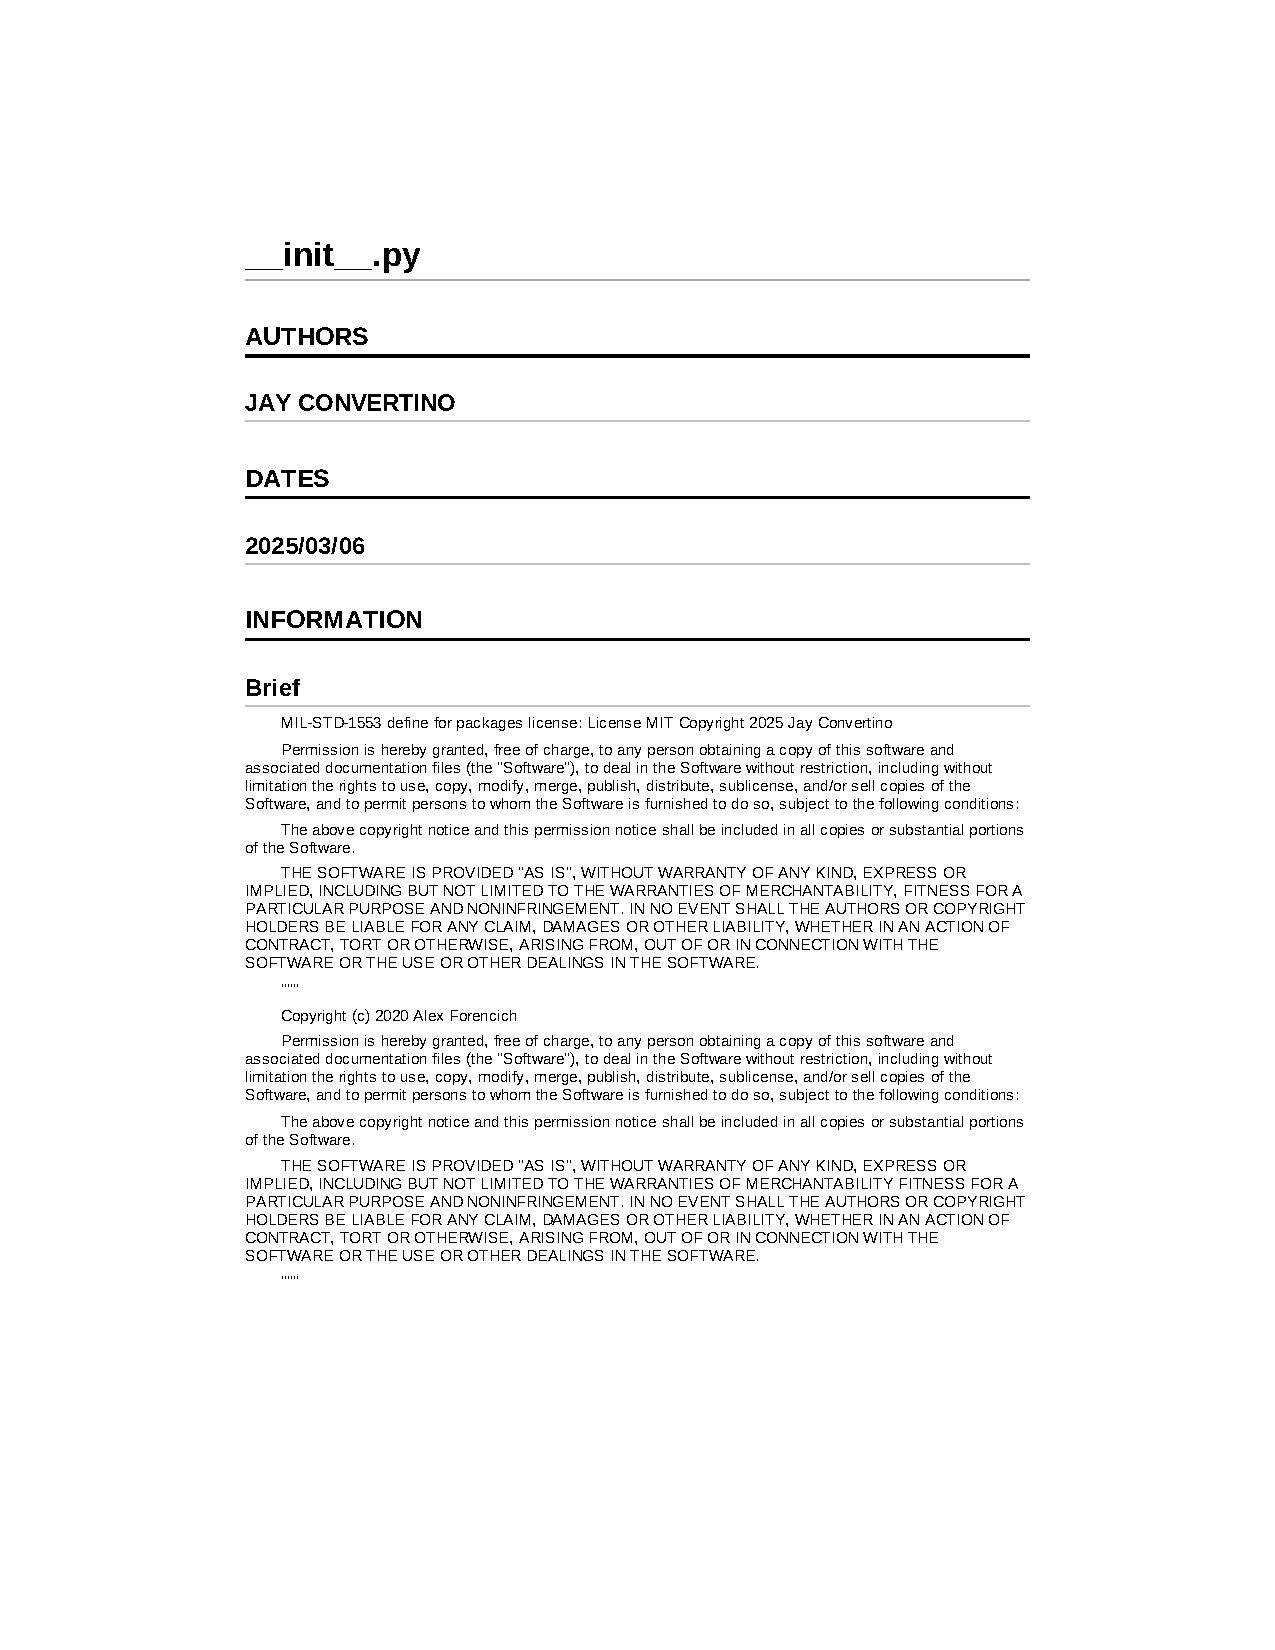
\includepdf[pages=-, addtotoc={1,subsection,1,init,p1}, pagecommand={}]{files___init__-py.pdf}
  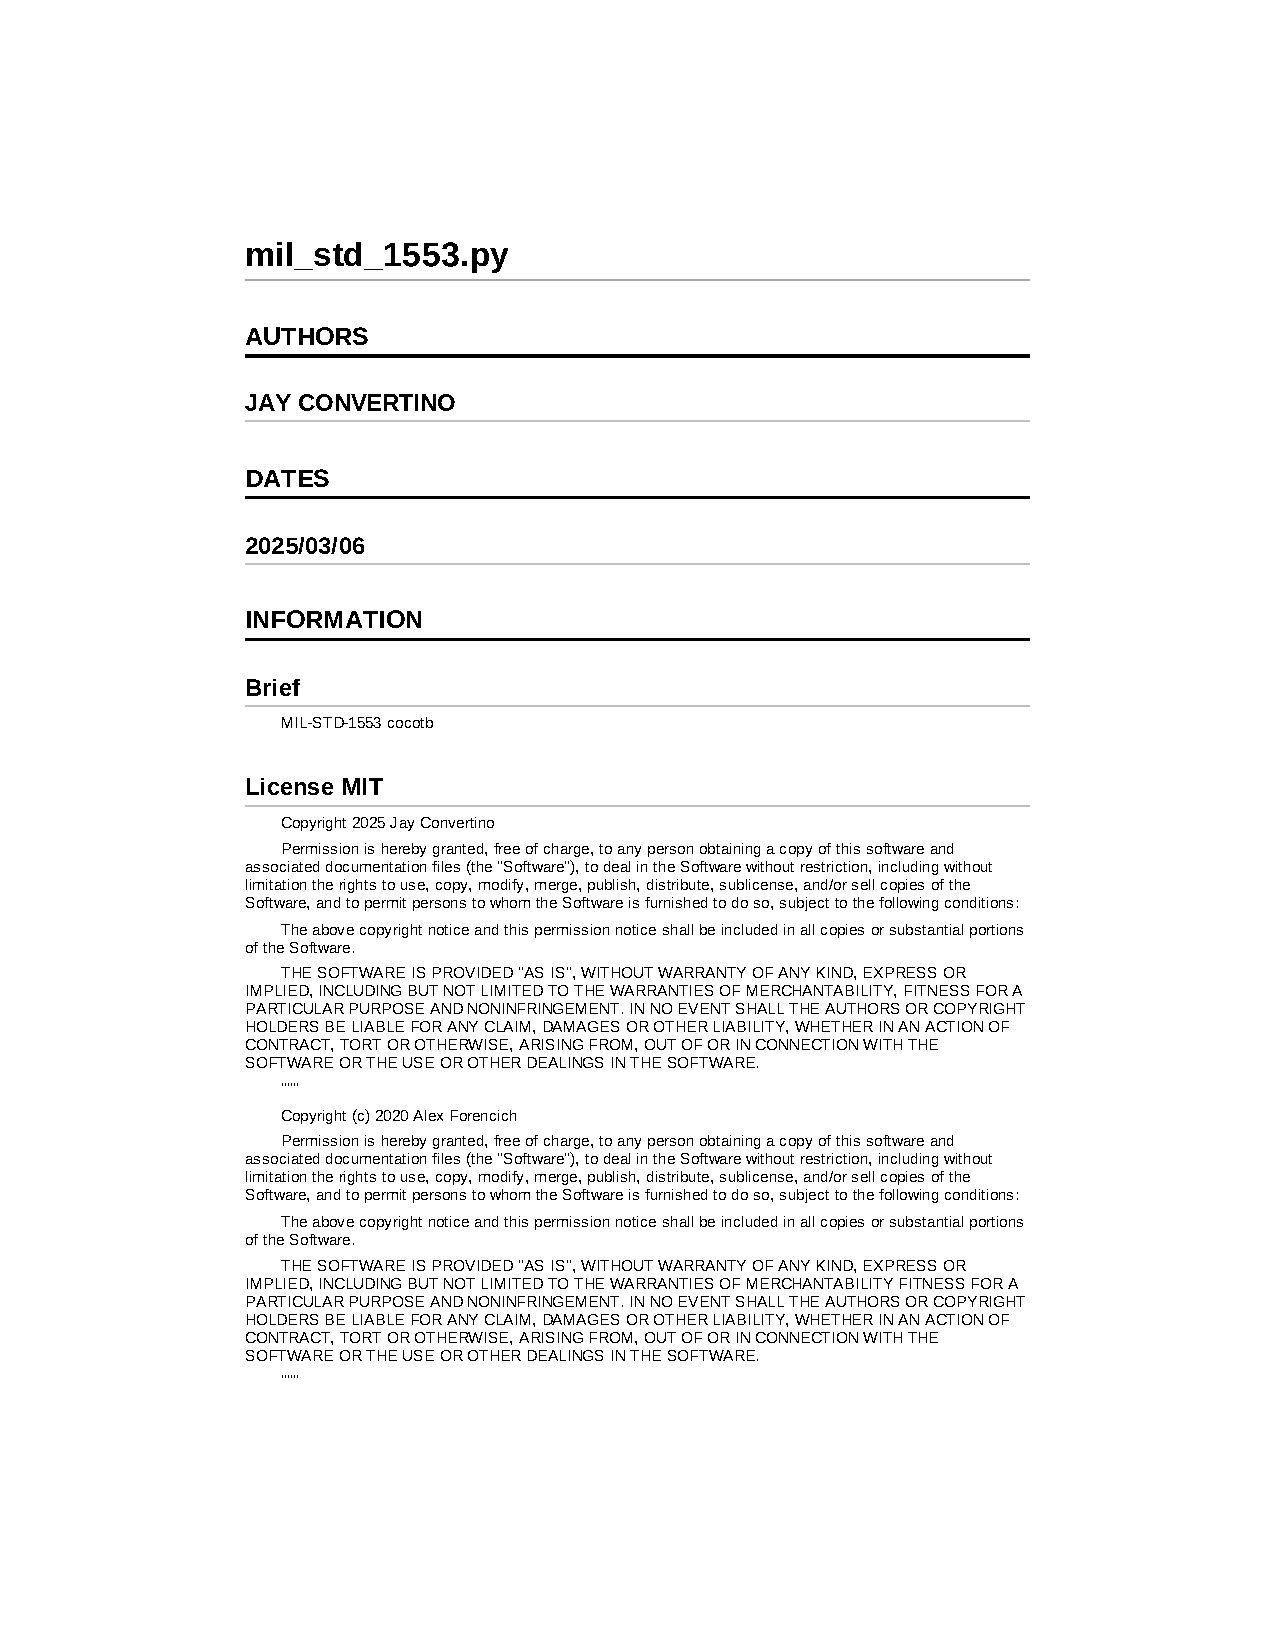
\includepdf[pages=-, addtotoc={1,subsection,1,mil-std-1553,p1}, pagecommand={}]{files_mil_std_1553-py.pdf}
  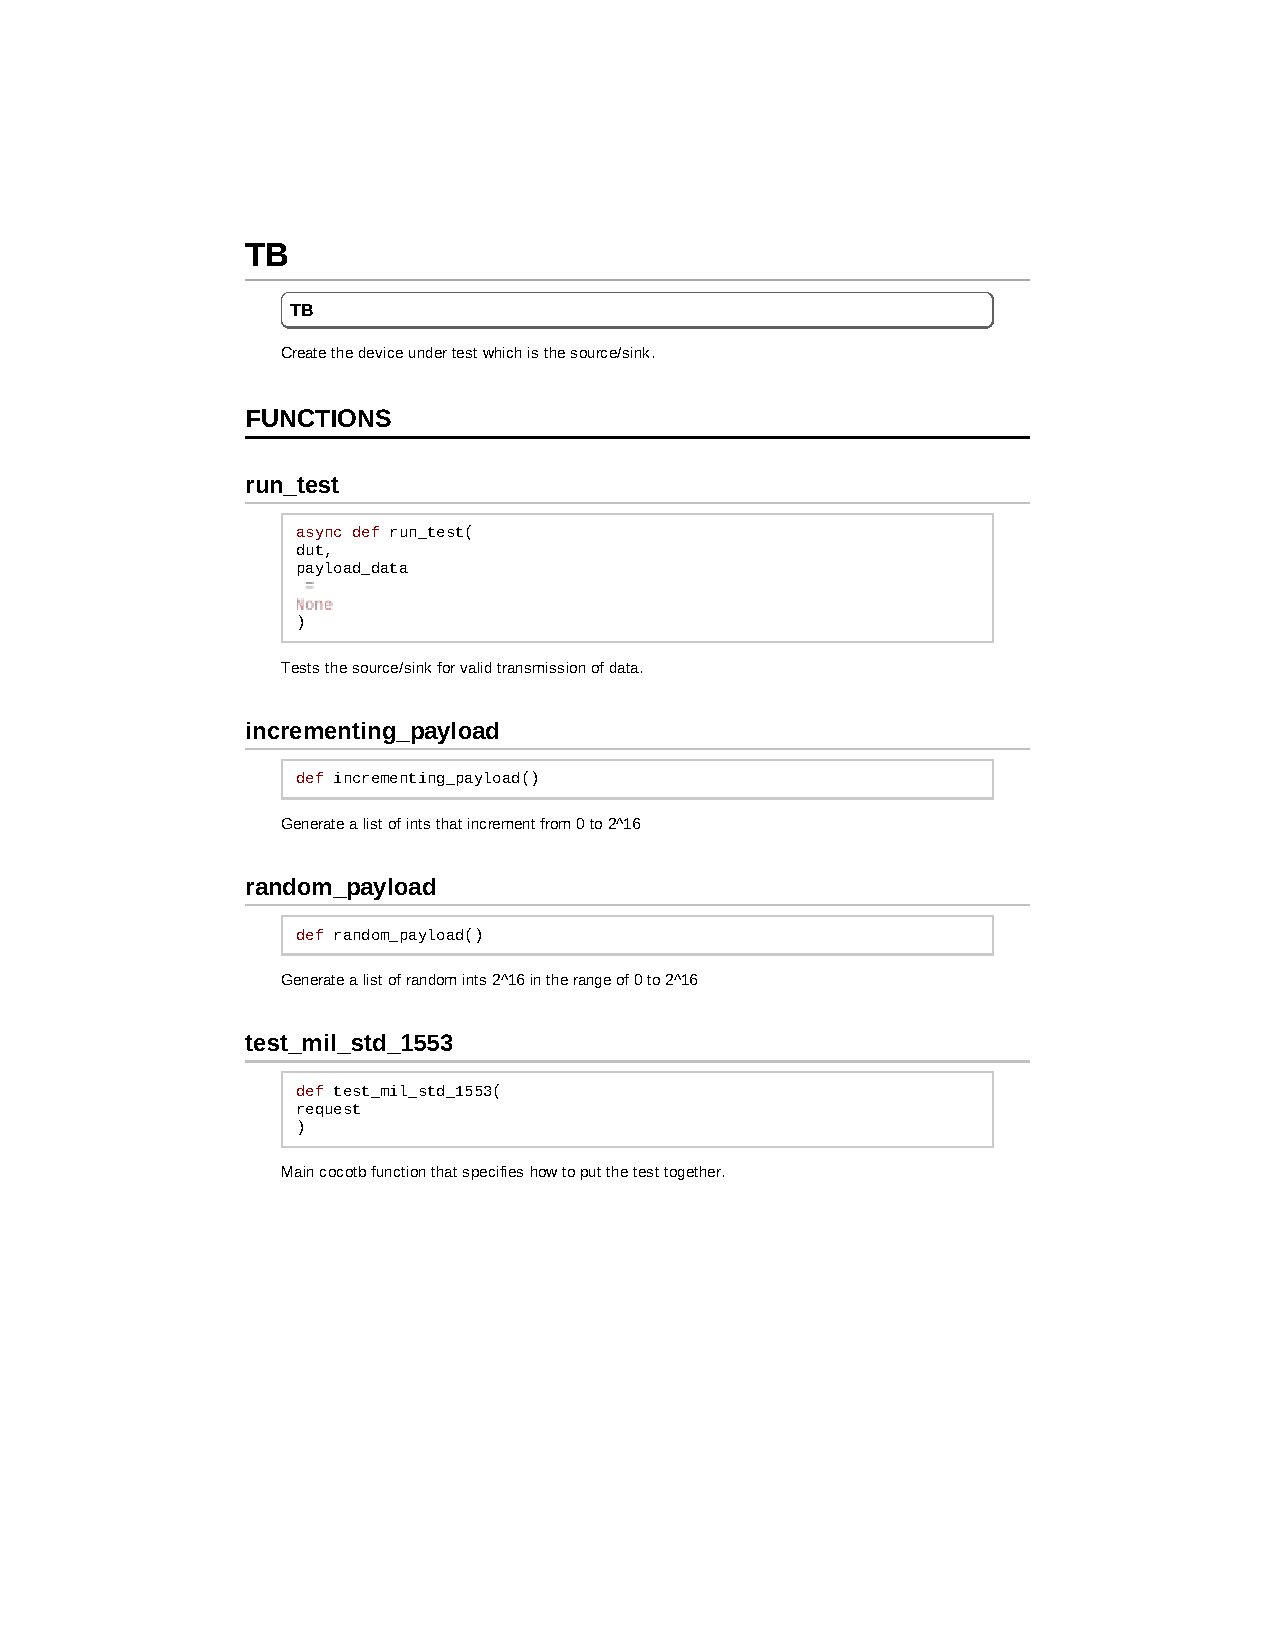
\includepdf[pages=-, addtotoc={1,subsection,1,test mil-std-1553 python,p1}, pagecommand={}]{files2_test_mil_std_1553-py.pdf}
  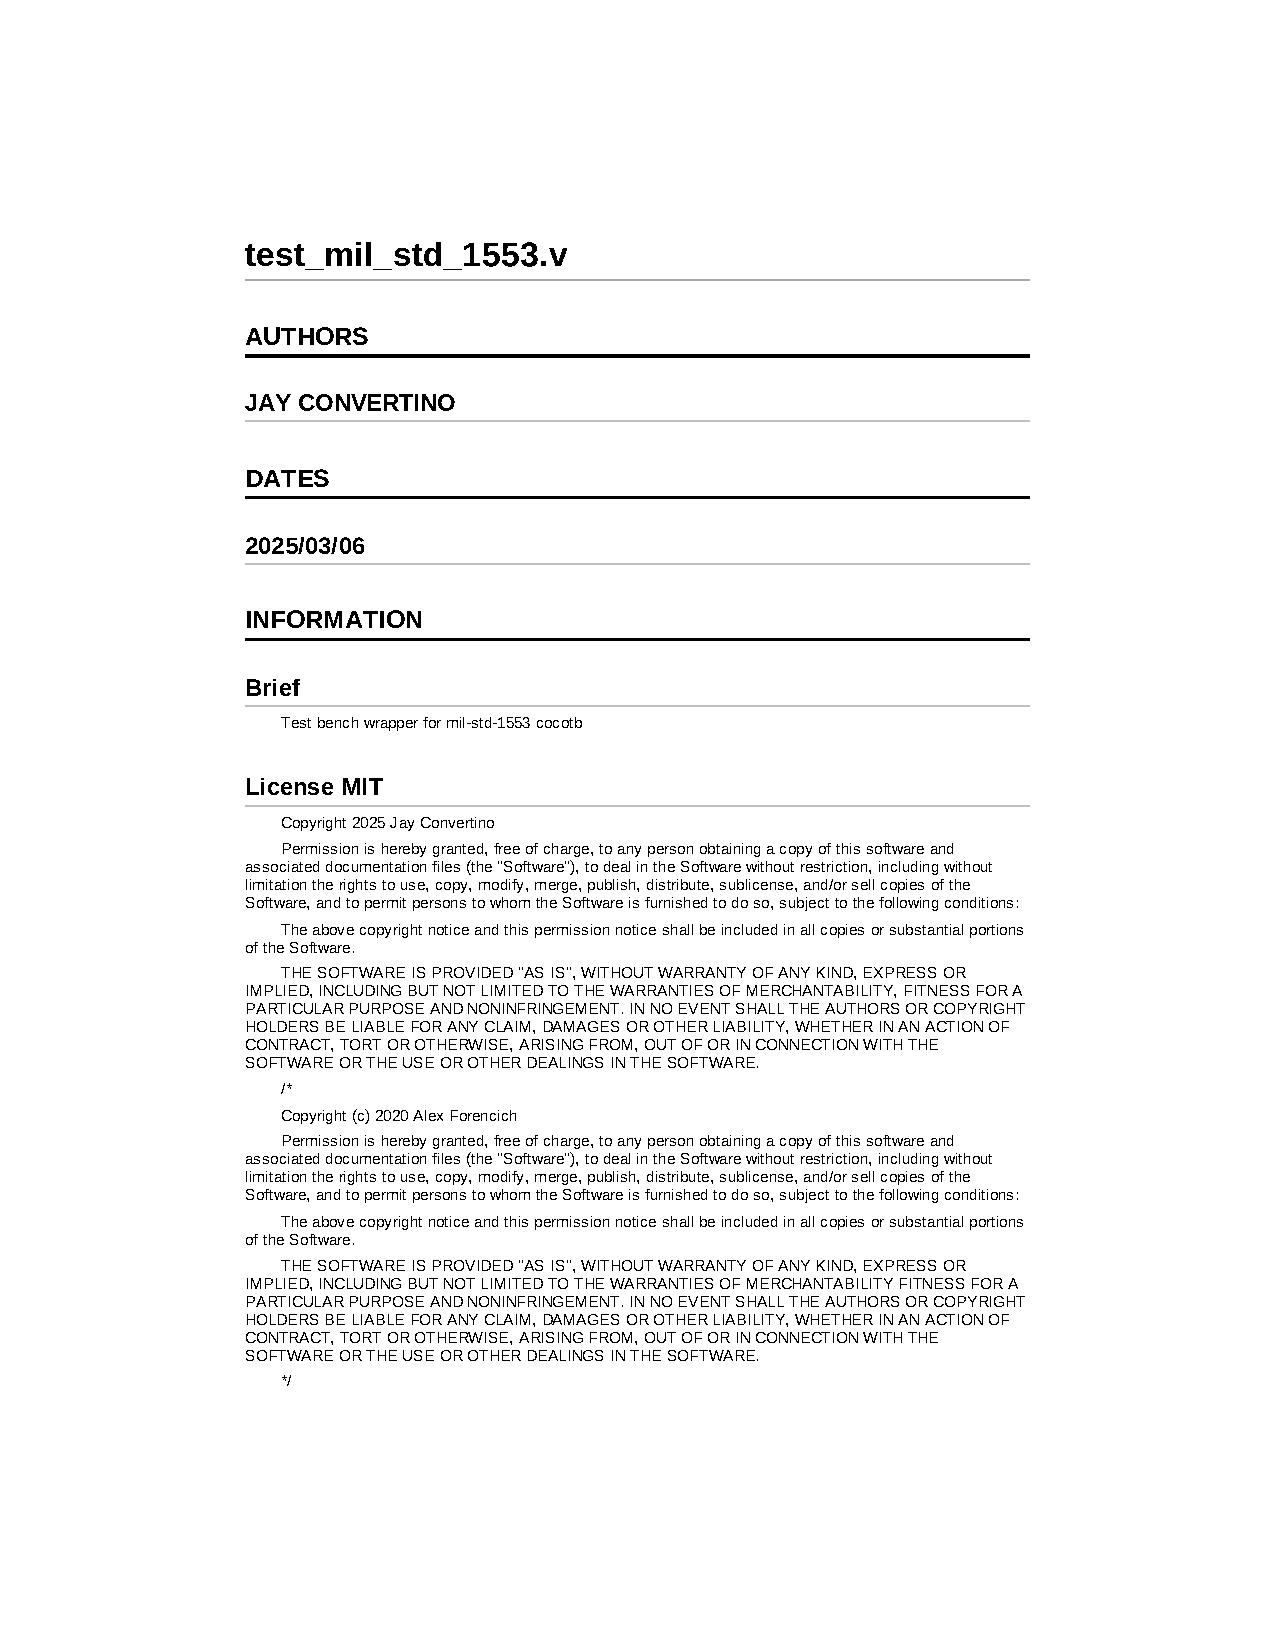
\includepdf[pages=-, addtotoc={1,subsection,1,test mil-std-1553 verilog,p1}, pagecommand={}]{files2_test_mil_std_1553-v.pdf}

\end{document}
